% Chapter 1

\chapter{Introduction} % Write in your own chapter title
\label{Chapter1}
\lhead{Chapter 1. \emph{Introduction}} % Write in your own chapter title to set the page header

\orange
\begin{shaded}
\subsection{Motivation}

SPolly, short for speculative Polly [TODO or \textbf{S}ambamba \textbf{Polly} :P],
is an attempt to combine two recent research projects in the context of compilers.
One the one hand side there is Polly, a LLVM project to increase data locality
and parallelism of loop nests. On the other hand there is Sambamba, which 
pursues a new, adaptive way of compiling and offers features like method 
versioning, speculation and runtime adaption. As an extension of the former one
and with the capabilities offered by the later one,
SPolly can perform state-of-the-art loop optimizations on a wide range of loops,
even in general purpose benchmarks as the SPEC 2000 benchmark suite. 

The presented results will show that speculative optimizations performed by
SPolly not only try to increase parallelism but also data locality --  two
bottlenecks of modern computation are tackled at the same time. 


\subsection{Overview}

This thesis is about the work on SPolly, a speculative loop optimizer based on
Polly and Sambamba. The key idea is to enable more loop optimizations due to 
speculation. To demarcate this from guessing, static and dynamic information 
is collected and used by an heuristic to choose promising candidates. 

The rest of the thesis will be organised as follows. 
The background theory and the tools SPolly is based 
on will be illustrated in chapter \ref{Chapter2}.
SPolly starts in chapter \ref{Chapter3} with the realization,
followed by an evaluation (chapter \ref{Chapter4}) on the SPEC 2000 and 
Polybench 3.2 benchmark suites. 
Chapter \ref{Chapter5} discusses the results in the context of
possible future work.
Before chapter \ref{Chapter7}
will conclude this thesis, a case study on different versions of the matrix 
multiplication example is presented in chapter \ref{Chapter6}. 

\end{shaded}


\begin{figure}[htbp]
  \centering
  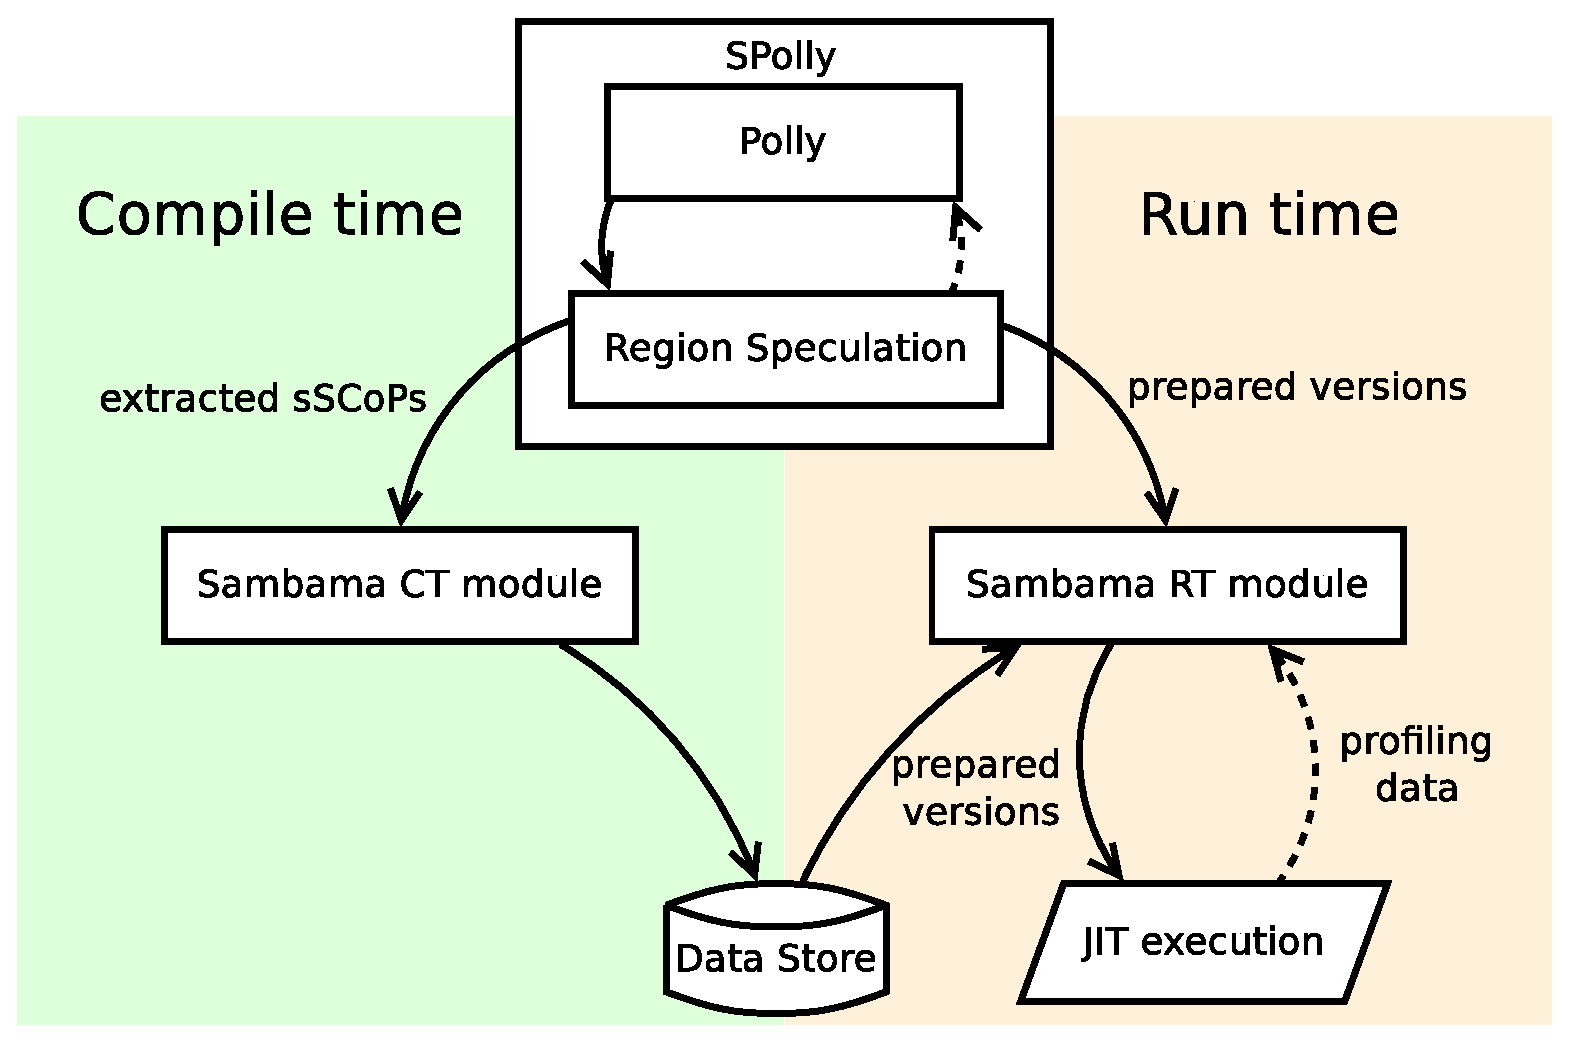
\includegraphics[width=0.9\textwidth]{Figures/Overview.eps}
  \caption{Overview [TODO]}
  \label{fig:Overview}  
\end{figure}
